\section{Istota programu}\label{tesliper:essence}
Zadaniem stworzonego przeze mnie oprogramowania jest wsadowe przetwarzanie plików wynikowych
  programu Gaussian\sidecite{gaussian09,gaussian16}, w~szczególności takich plików, które zawierają
  dane pochodzące z~optymalizacji struktury oraz obliczania jej aktywności optycznej\sidenote{
    Gaussian nie jest jedynym programem zdolnym do~przeprowadzenia takich obliczeń,
      jednak ograniczam się do~niego, gdyż jest on powszechnie stosowany.}.
Finalnym efektem działania \tesliper{}a jest symulowane widmo spektroskopowe badanego związku,
  powstałe przez uśrednienie teoretycznych widm każdego z~wybranych konformerów.
Program asystuje w~realizacji tych kroków procesu symulacji, które wymagają analizy danych
  ze~wspomnianych plików oraz w~przygotowaniu kolejnego etapu obliczeń.

\subsection{Proces symulacji widm}\label{essence:simulation}
Jak wywnioskować można z~poprzednich akapitów, symulacja widma spektroskopowego jest
  procesem kilkuetapowym.
Dokładnie opisują go \citeauthor{pescitelli16}, podając wskazówki i~sugerując dobrą
  praktykę w~tej pracy.\sidecite{pescitelli16}.
Na~potrzeby dyskusji zawartej w~niniejszej dysertacji poniższe ogólne przedstawienie
  stosowanej metodologi wydaje mi się wystarczające.

Punktem wyjścia jest proponowana konfiguracja absolutna badanego związku.
Należy poddać ją wnikliwej analizie konformacyjnej, to znaczy znaleźć możliwie dużo
  potencjalnie stabilnych konformerów związku o~zakładanej strukturze.
Dokonuje się tego zwykle za~pomocą dedykowanych programów komputerowych, operujących w~obrębie
  modelu mechaniki molekularnej.
Ich geometrie optymalizuje się korzystając z~metod \gls{dft}, a~później porównuje się ze~sobą,
  odrzucając duplikaty\sidenote{
    Zadarza się bowiem, że różne struktury uzyskane w~wyniku analizy konformacyjnej zostaną
      zoptymalizowane do~takiej samej geometrii.}.

Następnie należy przeprowadzić obliczenia częstości, aby potwierdzić, że uzyskane
  struktury są punktami stacjonarnymi, oraz obliczenia energii, niezbędnych do~przeprowadzenia
  analizy rozkładu Boltzmanna\sidenote{
    Prowadzącego do~oszacowania udziału każdego z~konforemrów w~populacji.}.
Jako, że kolejny etap obliczeń jest kosztowny\sidenote{W~sensie wymaganego czasu obliczeniowego.},
  zwykle liczbę wziętych do~niego konformerów ogranicza się, odrzucając te, które mają marginalny
  udział w~populacji.
Wtedy dopiero poddaje się pozostałe konformery obliczeniom wybranej aktywności spektroskopowej
  w~funkcji częstości albo długości falowej\sidenote{Zależnie od~typu symulowanego widma.}.
Wartości te nie są jeszcze symulowanym widmem.
Jego otrzymanie wymaga wykonania dalszej pracy \--- przeliczenia ich na~intensywność pików,
  symulacji kształtu pików, i~w~końcu uśrednienia uzyskanych w~ten sposób teoretycznych widm
  poszczególnych konformerów.

\begin{figure*}
  \includesvg{simulation-flow}
  \caption{
    Schemat przedstawiający proces symulacji widma spektroskopowego metodami numerycznymi.
    Zaznaczyłem na~nim etapy, które mogą zostać wykonane w~programie Gaussian i~autorskim
      programie \tesliper{}.
  }\label{fig:simulation-flow}
\end{figure*}

\Cref{fig:simulation-flow} przedstawia schematycznie ten proces, wyszczególniając kolejne etapy.
Jedynie niektóre z~tych etapów można wykonać za~pomocą programu do~obliczeń kwantowo-chemicznych,
  o~realizację pozostałych musi zadbać badacz.
Na~wspomnianym schemacie zaznaczam kolorowymi obszarami etapy, które mogą być zrealizowane
  w~programie Gaussian oraz te, w~których można użyć opisywanego programu \tesliper{}.

\subsection{Funkcje programu}\label{essence:features}
Przedstawiwszy ogólny przebieg typowego procesu symulacji widma spektroskopowego,
  mogę szczegółowo omówić funkcje, które \tesliper{} oferuje.
Jak wspomniałem we~wstępie do~tego rozdziału, oprócz samej symulacji widma, \tesliper{}
  dostarcza kilku dodatkowych funkcjonalności, pomocnych przy tym zadaniu.
Najważniejsze z~nich wymieniam poniżej.
Wszystkie one są realizowane w~trybie wsadowym\sidenote{%
  Warto może w~tym miejscu wyjaśnić ten termin szczegółowo.
  Wywodzi się on z~tradycyjnej klasyfikacji metod produkcji, w~której oznacza wytwarzanie
    określonej ilości produktów na~raz, zazwyczaj w~kilkuetapowym procesie.
  Do~użytku w~naukach komputerowyh wszedł już za~czasów komputerów sterowanych kartami
    dziurkowanymi, gdzie odnosił się do~systemu automatyzującego podawanie większej liczby
    takich kart komputerowi, wykonującemu określone zadanie.
  Tutaj używam go w~kontekście przetwarzania pewnej ilości plików lub danych
    według zadanych parametrów.
}.  

\begin{enumerate}
  \item Przeprowadzenie ekstrakcji danych z~plików wynikowych programu Gaussian.
    Odczytywanie i~przechowywanie jedynie tych danych, które są istotne z~punktu widzenia
      symulacji spektroskopowych pozwala na~wydajne i~szybkie przetwarzanie wskazanych plików.

  \item Obliczanie składu populacji konformerów metodą analizy Boltzmanna\sidenote{%
      Opisuję ją w~kolejnym rozdziale, w~sekcji~\secref{implementation:boltzmann}.
    }.
    Wykorzystywane do~tego są wartości energii konformerów obliczone przez program Gaussian.
    Otrzymane wartości mogą zostać użyte w~kolejnych krokach \--- selekcji konformerów:
      do~wykluczenia tych o~małym wkładzie oraz symulacji widm: do~ich uśrednienia.

  \item Wykluczanie konformerów niepodlegających dalszej analizie (selekcja).
    Dotyczy to zarówno prostego filtrowania obliczeń, które zakończyły się niepowodzeniem,
      albo konformerów, których nie udało się zoptymalizować, ale również bardziej złożonych
      operacji \--- na~przykład wykrywania struktur, które nie znajdują się w~lokalnym
      minimum energetycznym.
    Program \tesliper{} może również ograniczyć analizowane konformery do~takich, których
      pewna właściwość zawiera się w~danym przedziale \--- na~przykład których różnica
      energii względem konformeru najniżej energetycznego jest nie większa niż \SI{5}{\kcalpm}.

  \item Porównanie geometrii konformerów metodą matematyczną.
    Krok ten pozwala na~zminimalizowanie ilości podobnych do~siebie struktur, a~co za~tym idzie,
      zminimalizowanie poniesionych kosztów obliczeniowych.
    Program dokonuje tego porównując konformery metodą \gls{rmsd}\sidenote{%
      Detale na~ten temat również w~kolejnym rozdziale, w~sekcji~\secref{implementation:rmsd}.
    }.

  \item Przygotowanie kolejnego kroku obliczeń numerycznych.
    Polega ono na~utworzeniu szeregu plików tekstowych, po~jednym na~każdy analizowany konformer,
      zgodnych ze~specyfikacją plików wejściowych programu Gaussian.
    Po~wprowadzeniu do~pamięci \tesliper{}a pożądanych parametrów obliczeń,
      generuje on~takie pliki.

  \item Obliczanie symulowanego widma.
    Wychodząc z~aktywności obliczonych przez program Gaussian, \tesliper{} oblicza teoretyczne
      widmo dla każdego z~analizowanych konformerów, zgodnie z~zadanymi parametrami.
    Kształt pików symuluje za~pomocą funkcji Gaussa lub funkcji Lorentza\sidenote{%
      Ponownie, więcej na~ten temat w~kolejnym rozdziale, w~sekcji~\secref{implementation:spectra}.
    }.
    Otrzymany zestaw widm uśrednia według populacji otrzymanych w~wyniku analizy Boltzmanna.

  \item Zapis danych na~dysk twardy.
    Zarówno dane obliczone przez \tesliper{}, jak i~te odczytane z~plików wynikowych programu
      Gaussian, mogą zostać zapisane na~dysk twardy komputera w~wybranej formie.
    Dostępne są: format tekstowy \texttt{.txt}, danych oddzielonych przecinkami \texttt{.csv}
      oraz arkusza programu Excel \texttt{.xlsx}.
    Ponadto, komplet danych może zostać zachowany w~natywnym formacie \tesliper{}a
      i~bezstratnie odtworzony w~pamięci programu w~późniejszym czasie.
  
\end{enumerate}

\subsection{Korzystanie z~programu}\label{essence:use}
Dostęp do~oferowanych funkcji \tesliper{} umożliwia poprzez interfejs graficzny, jak
  i~programistyczny, pozwalając na~preferowaną przez użytkownika metodę komunikacji \---
  wizualną lub tekstową.
Przygotowana przeze mnie szczegółowa instrukcja korzystania z~programu obejmuje obydwa sposoby.
Po wytyczne odnośnie instalacji programu oraz jego uruchomienia również odsyłam do~tego
  dokumentu.
Jak wspomniałem już wcześniej, jest on dostępna w~Internecie\sidenote{%
    Pod adresem \href{https://tesliper.readthedocs.io/}{www.tesliper.readthedocs.io}.
  },
  a~także, w~formie pliku PDF, wśród materiałów dodatkowych dołączonych do~niniejszej dysertacji.
Zarówno interfejs, komunikaty programu, jak i~instrukcję, napisałem w~języku angielskim.

\begin{figure}
  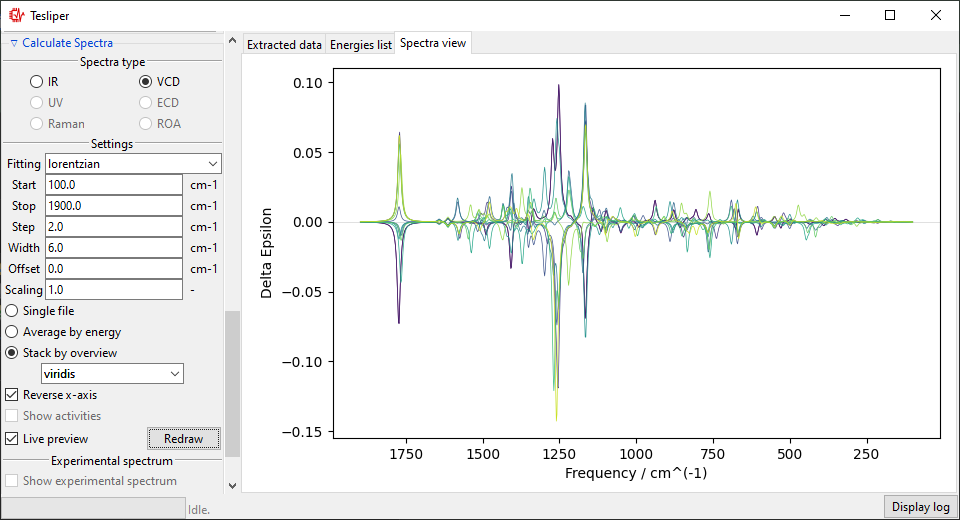
\includegraphics[width=\textwidth]{./chapter-4/essence/gui-demo}
  \caption{
    Przykład graficznego interfejsu programu \tesliper{} w~użyciu.
    W~oknie programu widoczne są nałożone na siebie teoretyczne widma \gls{vcd}
      wybranych konformerów.
    Po~lewej stronie widać panel kontrolek z~zadanymi parametrami symulacji widma.
  }
  \label{fig:gui-demo}
\end{figure}

W~tej sekcji chciałbym jedynie wstępnie przybliżyć sposób korzystania z~\tesliper{}a.
Na~\cref{fig:gui-demo} prezentuję wygląd jego interfejsu graficznego.
Zakładki na~górze okna pozwalają przełączać widok między kartami ukazującymi listę danych
  odczytanych dla każdego z~konformerów, listę wartości ich energii i~wartości pochodnych,
  i,~w~końcu, podgląd symulowanego widma.
Lewą stronę okna zajmuje panel z~kontrolkami pozwalającymi sterować programem \--- widocznych
  na~\cref{fig:gui-demo} jest tylko ich część, odpowiadająca za~parametry symulacji widma.
Nieujęte są te odpowiedzialne za~odczyt i~zapis danych oraz selekcję konformerów.

W~przypadku zarówno graficznego interfejsu, jak i~skryptów wykorzystujących interfejs
  programistyczny, porządek działań jest taki sam\sidenote{
    Z~tą tylko różnicą, że interfejs graficzny część akcji dodatkowo automatyzuje,
      na~przykład uśrednianie widma.}.
Pierwszym etapem jest zawsze wskazanie plików wynikowych programu Gaussian i~ich odczytanie
  przez \tesliper{}.
Następnie użytkownik możne porównać ze~sobą konformery i~dokonać ich selekcji według oczekiwań.
Kolejnym krokiem będzie obliczenie widm teoretycznych i~ich uśrednienie, a~w~końcu zapis
  wybranych danych na~dysk twardy komputera.
Przykład realizacji tego procesu poprzez interfejs programistyczny przedstawiam
  w,~opatrzonym komentarzami, \cref{lst:api-demo}.

\begin{listing*}
  \begin{lstlisting}[
    emph={input_dir, maximum, threshold, window_size, energy_genre, fmt}
  ]
    from tesliper import Tesliper  # dostęp do funkcjonalności teslipera
    
    # przetworzenie plików wyjściowych Gaussian
    tslr = Tesliper(input_dir="./opt_and_freq")
    tslr.extract()  # odczytaj wszystkie ze wskazanego folderu
    
    # selekcja konformerów do analizy
    # odrzuć konformery, których obliczenia nie zakończyły się normalnie
    tslr.conformers.trim_non_normal_termination()
    # a także te niezoptymalizowane
    tslr.conformers.trim_not_optimized()
    # oraz nie będące w lokalnym minimum energetycznym
    tslr.conformers.trim_imaginary_frequencies()
    # zatrzymaj konformery do +10 kcal względem najtrwalszego
    tslr.conformers.trim_to_range("gib", maximum=10, attribute="deltas")
    # porównaj geometrię i odrzuć duplikaty
    tslr.conformers.trim_rmsd(threshold=1, window_size=0.5, energy_genre="gib")
    
    # oblicz widma z dostępnych danych według standardowych parametrów
    tslr.calculate_spectra()
    # uśrednij obliczone widma teoretyczne według rozkładu Boltzmanna
    tslr.average_spectra()
    # zapisz wartości energii i pochodne do plików tekstowego
    tslr.export_energies(fmt="txt")
    # zapisz uśrednione widma do plików w formacie CSV
    tslr.export_averaged(fmt="csv")
  \end{lstlisting}
  \caption{Przykład skryptu wykorzystującego interfejs programistyczny \tesliper{}a.}
  \label{lst:api-demo}
\end{listing*}

\subsection{Podobne narzędzia}\label{essence:simmilar}
Program \tesliper{} nie jest jedynym programem z~graficznym interfejsem, który pozwala
  na~uzyskanie symulowanego widma spektroskopowego.
Dostępne są zarówno takie komercyjne, jak i~darmowe programy.
Do tych pierwszych zaliczyć można GausView\sidecite{gaussview} dedykowany pracy z~programem
  Gaussian, dostarczany przez producenta sprzętu spektroskopowego ComputeVOA\sidecite{computevoa},
  oraz niezależny ChemCraft\sidecite{chemcraft}.
Bezpłatne są natomiast programy przygotowane przez społeczność naukową \---
  CDspecTech\sidecite{cdspectech} oraz SpecDis\sidecite{specdis}.

Na tle ich wszystkich \tesliper{} wyróżnia się otwartością kodu źródłowego \---
  użytkownik ma wgląd w~jego strukturę i~detale implementacji.
Model ten ma szereg zalet, jak choćby przejrzystość kodu i~wynikające z~niej niezawodność
  i~bezpieczeństwo \--- każdy może upewnić się, że działanie programu jest zgodne z~jego opisem,
  poznać sposób jego funkcjonowania, zaproponować poprawki i~usprawnienia.
Unikalną cechą \tesliper{}a jest funkcja selekcji konformerów, to znaczy dopuszczenia do~analizy
  tylko konformerów o~zadanych przez użytkownika właściwościach.
Pozwala to na~łatwe odrzucenie błędnych wyników obliczeń, czy zawężenie puli struktur do~najniżej
  energetycznych.

\begin{table*}
  \renewcommand{\arraystretch}{1.2}
  \setlength{\tabcolsep}{5pt}
  \begin{tabular}{ r *{6}{c} }
                 & \tesliper{} & GaussView & ComputeVOA & CDspecTech & ChemCraft & SpecDis \\
    Darmowy                    & \markok & \markno & \markno & \markok & \markno & \markok \\ 
    Otwartoźródłowy            & \markok & \markno & \markno & \markno & \markno & \markno \\
    Wieloplatformowy\tsp{a}    & \markok & \markok & \markno & \markno & \markpm\tsp{b} & \markok \\
    Przetwarzanie wsadowe      & \markok & \markpm\tsp{c} & \markno & \markok & \markpm\tsp{d} & \markno \\
    Porównanie geometrii       & \markok & \markno & \markok & \markno & \markok & \markno \\
    Rozkład Boltzmanna         & \markok & \markno & \markno & \markok & \markno & \markok \\
    Selekcja konformerów       & \markok & \markno & \markno & \markno & \markno & \markno \\
    Przygotowanie obliczeń     & \markok & \markok & \markok & \markno & \markok & \markno \\
    Widma elektronowe          & \markok & \markok & \markno & \markok & \markno & \markok \\
    Widma ramanowskie          & \markok & \markok & \markok & \markok & \markok & \markno \\
    Analiza konformacyjna      & \markno & \markpm\tsp{e} & \markok & \markno & \markno & \markno \\
  \end{tabular}
  \caption{
    Porównanie różnych programów oferujących interfejs graficzny, które pozwalają na~symulację
      widm z~plików wynikowych programu Gaussian.
    Otwartość kodu źródłowego i~funkcja warunkowego wyboru konformerów są unikalnymi cechami
      autorskiego programu \tesliper{}.
    \tsp{a}Czyli funkcjonuje na~różnych systemach operacyjnych.
    \tsp{b}Wymaga użycia dodatkowego oprogramowania.
    \tsp{c}Tylko masowy eksport plików wejściowych.
    \tsp{d}Tylko masowa modyfikacja plików wejściowych.
    \tsp{e}Dostępne jako dodatkowy moduł.
  }
  \label{tab:comparison}
\end{table*}

\Cref{tab:comparison} zawiera porównanie tych programów pod kątem funkcjonalności, jakie oferują.
Poza kwestią unikalnych cech \tesliper{}a, wymienione aplikacje mają też inne istotne braki,
  choćby w~kwestii ich dostępności na~różnych systemach operacyjnych.
Oprócz \tesliper{}a, jedynie CDspecTech zapewnia wsadowe przetwarzanie danych w~pełnym zakresie
  oferowanej funkcjonalności \--- w~pozostałych aplikacjach jest ono niemożliwe
  lub znacznie ograniczone.
Nie wszystkie są też w~stanie przeprowadzić pełną symulację widma, włącznie z~uśrednianiem
  danych z~analizy poszczególnych konformerów.
Funkcją, której nie oferuje \tesliper{} jest natomiast analiza konformacyjna \--- do~jej
  przeprowadzenia zdolne sią jedynie niektóre programy komercyjne.
